%  MDPI Sensors — Journal Submission Draft
%  Title: Trustworthy Field sEMG Fatigue Monitoring on a Low-Cost Wearable
%  Status: DRAFT — §6.7 and full abstract pending N3 multi-subject data

\documentclass[sensors,article,submit,pdftex,moreauthors]{Definitions/mdpi}

% Internal metadata
\firstpage{1}
\makeatletter
\setcounter{page}{\@firstpage}
\makeatother
\pubvolume{1}
\issuenum{1}
\articlenumber{0}
\pubyear{2026}
\copyrightyear{2026}
\datereceived{ }
\daterevised{ }
\dateaccepted{ }
\datepublished{ }

\conference{Extended from: (1) R. Wang, T. Di, Y. Di, ``Field Validity of Wearable sEMG
Fatigue Metrics in Tennis,'' CNIB, 2026; (2) R. Wang, ``A Robust Self-Describing BLE
Platform for Real-Time Wearable EMG--IMU Sensing,'' ICPICS, 2026.}

%=============================================================
% Title
%=============================================================
\Title{Trustworthy Field sEMG Fatigue Monitoring on a Low-Cost Wearable:
Electrode Settling, IMU-Conditioned Validity, and Continuity Auditing
on a \$99 ESP32 Platform}

% ORCID (add when available)
\newcommand{\orcidauthorA}{0000-0000-0000-0000}

%=============================================================
% Authors and Affiliations
%=============================================================
\Author{Ryan Wang $^{1}$\orcidA{}, Theodore Di $^{2}$ and YanMing Di $^{3,}$*}

\AuthorNames{Ryan Wang, Theodore Di and YanMing Di}

\address{%
$^{1}$ \quad Westview High School, San Diego, CA 92131, USA; ryanwang2020@gmail.com\\
$^{2}$ \quad Crescent Valley High School, Corvallis, OR 97330, USA; theodore.l.di@gmail.com\\
$^{3}$ \quad Oregon State University, Corvallis, OR 97331, USA}

\corres{Correspondence: Yanming.Di@oregonstate.edu}

%=============================================================
% Abstract (~200 words, no subheadings per MDPI Sensors)
%=============================================================
\abstract{Wearable surface electromyography (sEMG) promises objective fatigue
monitoring in field sports, but deployment is undermined by electrode settling,
contact-quality drift, and wireless session gaps. We present a low-cost (\$99~USD)
ESP32-based EMG--IMU wearable achieving 2000~Hz EMG and 200~Hz IMU BLE streaming,
paired with a trustworthiness-first methodology for no-gel tennis forearm fatigue
monitoring. The platform achieves $\pm$25~$\mu$s per-sample timestamp accuracy
(99.03\% over 7.5 million samples) via DMA oversampling, a self-describing BLE TLV
protocol surviving three firmware revisions, and a hybrid \textit{abs\_us} timeline
validated at $\pm$25~$\mu$s intra-connection and p99 $\leq$ 170~ms cross-connection.
In a 63.1-min field session (626 swings), median frequency (MDF) followed a
three-phase settling--reference--fatigue trajectory (115.7 $\rightarrow$ 167.6
$\rightarrow$ 149.5~Hz) visible only with $\geq$20~min warmup exclusion; a 10-min
skip missed the fatigue signal entirely ($-$2.6\% vs. $+$28.1\% at 20~min). IMU
swing intensity remained flat ($r = +0.029$, $p = 0.468$), excluding reduced effort.
IMU-guided pre-impact MDF windowing produced a mean $+$26.7~Hz shift versus
full-window MDF (81\% of swings), confirming physiologically motivated temporal
partitioning. A BLE reconnection gap created an apparent 28.7\% spurious fatigue
signal that collapsed to 4.9\% for the continuous segment. These findings establish
a platform--methodology framework requiring settling-aware baselines,
IMU-conditioned validity, and continuity auditing for trustworthy wearable sEMG
fatigue monitoring.}

\keyword{surface EMG; fatigue monitoring; electrode settling; IMU; wearable sensors;
BLE; ESP32; tennis; field deployment; DMA sampling}

%=============================================================
\begin{document}
%=============================================================

%%%%%%%%%%%%%%%%%%%%%%%%%%%%%%%%%%%%%%%%%%
\section{Introduction}
\label{sec:intro}

Surface electromyography (sEMG) can quantify local muscle fatigue through spectral
metrics such as median frequency (MDF) and mean frequency (MNF), which shift toward
lower values as motor unit conduction velocity decreases with metabolite accumulation.
Tennis players can often perceive general tiredness, but subjective perception is not a
quantitative, muscle-specific measure of local fatigue. Objective EMG monitoring may
complement perception by enabling session-to-session workload tracking and future
overuse-risk assessment; upper-extremity tennis injuries are frequently chronic and
repetitive, with lateral elbow tendinopathy associated with repeated forearm muscle
loading~\cite{aaos2023}.

In real court deployment, gel electrode preparation is impractical: gel smears during
play, affects racket grip, and players resist pre-session preparation. This study
intentionally evaluates a no-added-gel, field-deployable configuration because routine
on-court monitoring requires fast setup and minimal interference with play, contrasting
with SENIAM-style laboratory preparation~\cite{hermens2000}. In this setting,
electrode--skin impedance starts high and decreases over time as sweat hydrates the
interface---a process that can make short fixed warmup exclusions insufficient.

Commercial research-grade systems (e.g., Delsys Trigno~\cite{delsys2024}, Noraxon
Ultium~\cite{noraxon2024}) capture EMG and IMU reliably but at \$5{,}000--\$30{,}000
per unit are out of reach for youth sport and most field research. Low-cost alternatives
based on commodity microcontrollers face three practical challenges: (i)~achieving
2000~Hz EMG sampling without sample loss requires careful ADC architecture;
(ii)~reliable BLE streaming at the combined EMG + IMU data rate demands efficient
packetization and reconnection handling; and (iii)~multi-sensor systems require precise
timestamp alignment across sensors with different sampling rates
(2000~Hz vs. 200~Hz)~\cite{cerone2019,lynn2018,yang2024}.

Existing IMU--EMG wearable studies typically fuse both modalities as feature sources for
activity or fatigue classification~\cite{taborri2020,bangaru2022}. In contrast, this
work uses the IMU as an \textbf{independent biomechanical context sensor} for EMG
validity assessment. Because tennis swings generate repeatable forearm kinematic
signatures, stable IMU swing intensity provides a reference: when EMG changes while
IMU is stable, the cause---electrode settling, contact degradation, or local muscle
fatigue---can be inferred from temporal context.

The contributions of this work are:
\begin{itemize}
  \item[(C1)] Field characterization of electrode settling ($\geq$17--20~min,
    no-gel forearm snap electrodes);
  \item[(C2)] Warmup-skip sensitivity as a required robustness audit for no-gel field sEMG;
  \item[(C3)] Contact-quality-aware EMG interpretation via ENV/RAW amplitude ratio proxy;
  \item[(C4)] IMU-conditioned EMG validity framework (Table~\ref{tab:validity});
  \item[(C5)] Session-gap artifact detection via hybrid \textit{abs\_us} timeline auditing;
  \item[(C6)] \$99 ESP32 platform: DMA oversampling, self-describing TLV, two-layer watchdog;
  \item[(C7)] Quantitative \textit{abs\_us} hybrid timeline validation ($\pm$25~$\mu$s
    intra-connection, p99 $\leq$ 170~ms inter-connection);
  \item[(C8)] IMU-guided pre-impact MDF window (Approach~B, physiologically motivated).
\end{itemize}

%%%%%%%%%%%%%%%%%%%%%%%%%%%%%%%%%%%%%%%%%%
\section{Related Work}
\label{sec:related}

\subsection{Field vs. Laboratory sEMG Fatigue in Tennis}

The majority of sEMG fatigue studies use laboratory settings with controlled contractions,
gel electrodes, and stationary subjects. SENIAM guidelines~\cite{hermens2000} address
gel-electrode placement and signal quality but were developed for controlled configurations;
forearm placement during dynamic sport is not addressed.

Rota et al.~\cite{rota2014} measured upper limb EMG during sustained tennis rally play
using gel electrodes and a commercial Bagnoli system, reporting progressive MDF decline
in wrist extensors over $\sim$25~min. Wang et al.~\cite{wanglh2019} examined forearm
muscle fatigue and skill-level effects on serve ball speed using gel-electrode sEMG.
Girard et al.~\cite{girard2011} examined spinal and peripheral fatigue components during
prolonged tennis using neuromuscular testing at rest intervals. None of these works
addressed electrode settling artifacts, contact-quality monitoring, or timestamp
continuity; their laboratory settings made these unnecessary.

\textbf{Gap.} No prior work has characterized sEMG MDF fatigue trajectories under
no-gel field conditions with online swing detection, contact-quality monitoring, or
IMU-conditioned validity classification.

\subsection{Dry Electrode and Contact Quality}

Dry electrodes are required for rapid field deployment. Joutsen et al.~\cite{joutsen2024}
showed that skin--electrode impedance decreases as sweat accumulates over time,
providing the physical basis for the Phase~I settling we report. Boyer et
al.~\cite{boyer2023} reviewed noise and artifact reduction in single-channel EMG,
including dry electrode contact quality. Ravichandran et al.~\cite{ravichandran2023}
characterized dry e-textile electrode impedance properties under contact force and
perspiration, showing systematic interface impedance reduction with sweat accumulation.

\subsection{IMU + EMG Integration}

Taborri et al.~\cite{taborri2020} surveyed IMU + EMG integration in sports biomechanics;
most fusion approaches treat the IMU as a signal source to be combined with EMG at the
feature level. Our ``IMU-as-context'' framework (Section~\ref{sec:imu_cond}) uses the
IMU instead as a validity classifier and window selector. Bangaru et
al.~\cite{bangaru2022} used IMU + EMG for construction-worker fatigue in a field
setting, but their capture infrastructure did not require the engineering described here.

\subsection{Wearable EMG--IMU Platforms}

Table~\ref{tab:comparison} compares the platform developed in this work against
representative commercial and academic wearable EMG systems.

\begin{table}[H]
\caption{Engineering comparison of wearable EMG platforms for field deployment.
\label{tab:comparison}}
\begin{adjustwidth}{-\extralength}{0cm}
\begin{tabularx}{\fulllength}{p{2.8cm}p{1.8cm}p{1.3cm}p{1.3cm}p{1.5cm}p{2.2cm}p{2.2cm}p{1.6cm}p{1.3cm}}
\toprule
\textbf{Platform} & \textbf{Cost (USD)} & \textbf{EMG $f_s$ (Hz)} & \textbf{IMU $f_s$ (Hz)} & \textbf{Raw EMG} & \textbf{BLE Robustness} & \textbf{Timeline Recon.} & \textbf{Platforms} & \textbf{Open} \\
\midrule
This work (ESP32) & $\sim$\$99 & 2000 & 200 & Yes (RAW+ENV) & Self-describing TLV, CRC, two-layer watchdog & \textit{abs\_us}: $\pm$25~$\mu$s intra, p99 $\leq$170~ms inter & PC + Android & Yes \\
\midrule
Delsys Trigno \cite{delsys2024} & \$5--30K & 2000 & 148.1 & Proprietary & Proprietary RF & Proprietary & PC only & No \\
Noraxon Ultium \cite{noraxon2024} & \$5--20K & 2000 & 200 & Proprietary & Proprietary BLE & Proprietary & PC only & No \\
Cerone HD-sEMG \cite{cerone2019} & Research & 2048 & --- & Yes (HD) & Undocumented & Not documented & PC & Partial \\
Lynn/Athos \cite{lynn2018} & \$0.5--2K & 200 & Yes & ENV only & Closed system & Not documented & Mobile & No \\
Yang e-textiles \cite{yang2024} & Varies & Varies & Varies & Depends & Not documented & Not documented & Varies & Research \\
MultiSenseBadminton \cite{seong2024} & \$0.5--1K & --- & 200--1000 & --- & Not documented & Camera sync & PC & Dataset \\
\bottomrule
\end{tabularx}
\end{adjustwidth}
\end{table}

Key differentiators: \$99 cost vs. \$5{,}000--\$30{,}000 for research-grade systems;
simultaneous RAW+ENV access enabling spectral fatigue analysis; self-describing TLV
so FSR changes do not require host decoder updates; quantified \textit{abs\_us} timeline
accuracy (Section~\ref{sec:absus_val}); full PC+Android feature parity.

%%%%%%%%%%%%%%%%%%%%%%%%%%%%%%%%%%%%%%%%%%
\section{The \$99 ESP32 EMG--IMU Platform}
\label{sec:platform}

\subsection{Hardware and Bill of Materials}

The system uses five components totaling approximately \$99~USD (Table~\ref{tab:bom}).
The MyoWare~2.0 muscle sensor provides both a hardware-rectified envelope output (ENV)
and a raw AC-coupled output (RAW) on separate pins, essential for concurrent amplitude
and spectral EMG analysis.

\begin{table}[H]
\caption{Bill of materials.\label{tab:bom}}
\begin{tabularx}{\textwidth}{XCCR}
\toprule
\textbf{Component} & \textbf{Function} & \textbf{Rate} & \textbf{Cost (USD)} \\
\midrule
MyoWare 2.0 & EMG (ENV + RAW) & 2000~Hz & \$40 \\
ICM-20948 & 6-axis IMU & 200~Hz & \$15 \\
MAX30105 & SpO2/HR (optional) & $\sim$0.03~Hz & \$10 \\
MAX17048 & Battery fuel gauge & 0.1~Hz & \$5 \\
ESP32 WROOM-32E & MCU + BLE, 240~MHz dual-core & --- & \$12 \\
PCB / battery / wiring & Integration & --- & $\sim$\$17 \\
\midrule
\textbf{Total} & & & $\approx$\textbf{\$99} \\
\bottomrule
\end{tabularx}
\end{table}

The REF electrode is placed over the lateral epicondyle~\cite{sparkfun2023}. The
RAW signal is routed via a direct solder bypass from the MyoWare PTH pad to ESP32
GPIO~32, correcting a field-discovered pogo-pin routing failure described in
Section~\ref{sec:pogo}.

\subsection{Dual-Core FreeRTOS Architecture}

The ESP32 dual-core architecture enables strict separation of real-time sensor
acquisition from BLE protocol processing (Figure~\ref{fig:arch}).

\begin{figure}[H]
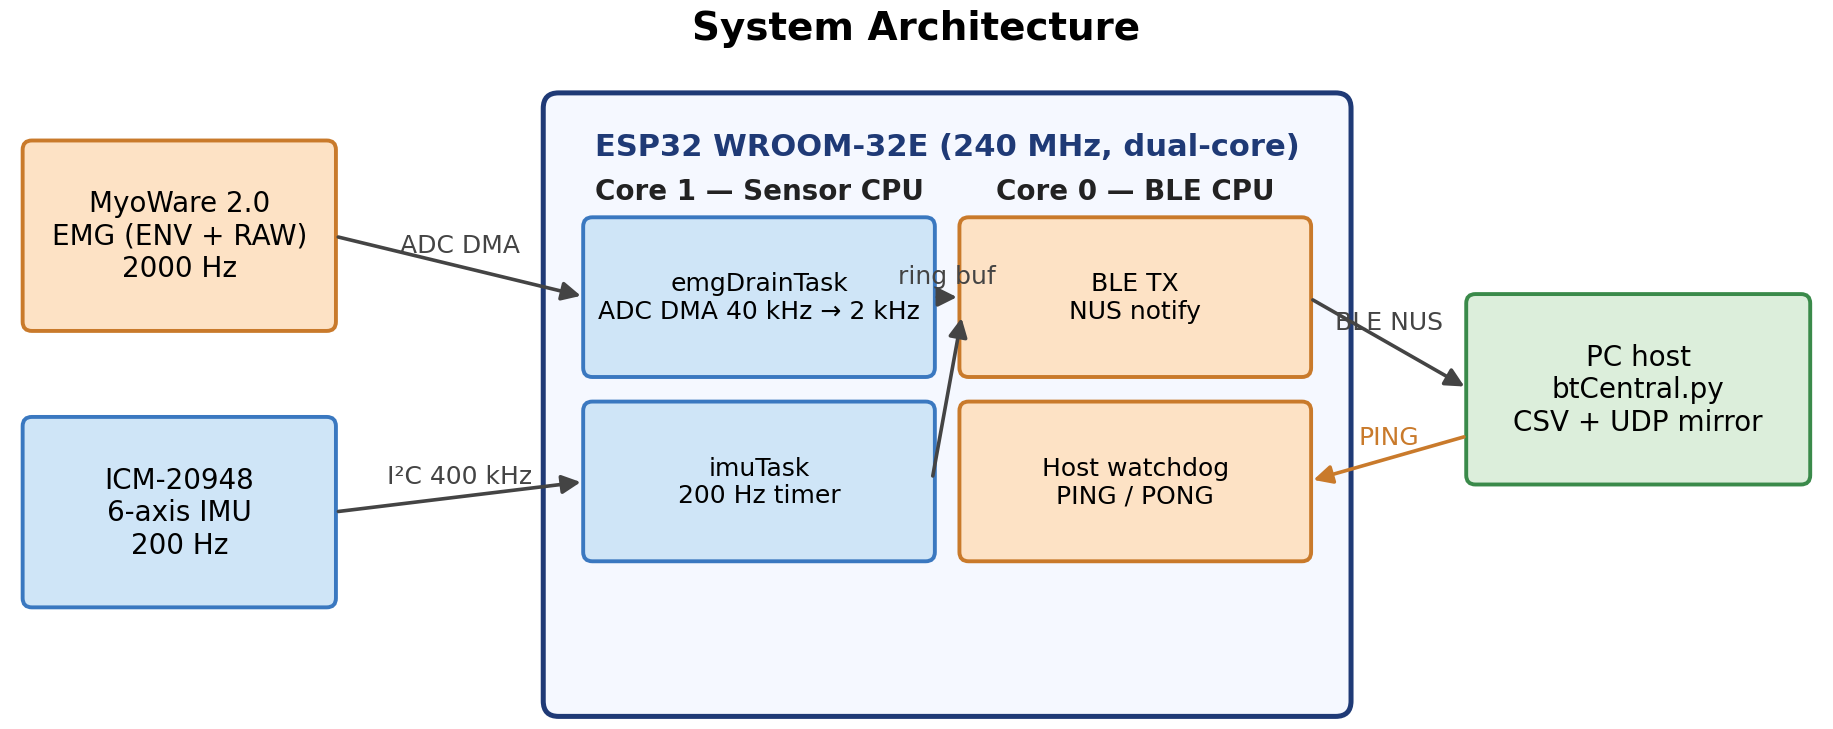
\includegraphics[width=\textwidth]{../icpics_figures/fig_system_architecture.png}
\caption{System architecture showing dual-core FreeRTOS task allocation, sensor
connections, and host interfaces. Core~1 (Sensor CPU) handles \texttt{emgDrainTask}
(priority~2), \texttt{imuTask} (priority~2), and \texttt{spo2Task} (priority~0).
Core~0 (Protocol CPU) handles BLE notifications, host watchdog, and LED state
machine.\label{fig:arch}}
\end{figure}

Task priority~2 for both \texttt{emgDrainTask} and \texttt{imuTask} was selected after
observing that priority~1 allowed \texttt{spo2Task} I2C operations to occasionally
starve IMU reads---a non-obvious FreeRTOS interaction documented here for other
practitioners.

\subsection{ADC DMA Oversampling and Timestamp Accuracy}

Timer-based ADC sampling at 2000~Hz would require 2000 interrupt service requests per
second per channel, competing with FreeRTOS scheduling. Instead, the ESP32 ADC
Continuous (DMA) driver runs at 40{,}000 conversions/s across both channels
(20{,}000/s per channel); \texttt{emgDrainTask} applies 10$\times$ software decimation
to produce the 2000~Hz output.

Per-sample timestamps are back-calculated from DMA frame completion time:
\begin{equation}
t_{i} = t_{\text{frameEnd}} - (N \times T_{\text{EMG}}) + (i \times T_{\text{EMG}})
\end{equation}
where $T_{\text{EMG}} = 500~\mu\text{s}$ (2000~Hz period) and $N$ is the number of
samples in the frame. This corrects for FreeRTOS scheduling jitter (up to 16~ms).

Empirical validation across 2.3~million samples confirms 99.03\% within $\pm$25~$\mu$s
of the expected 500~$\mu$s interval (Figure~\ref{fig:timing}, Table~\ref{tab:timing});
outliers at p99.9 (925~$\mu$s) correspond to brief BLE TX bursts ($<$0.1\% of samples).

\begin{figure}[H]
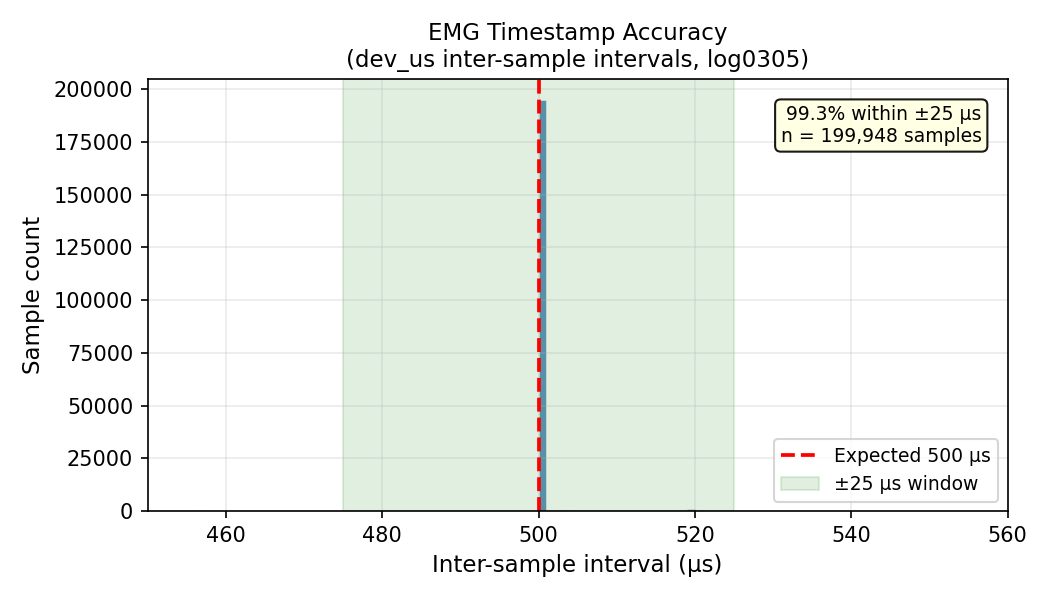
\includegraphics[width=0.75\textwidth]{../icpics_figures/fig_timing_accuracy.png}
\caption{Inter-sample interval distribution across 2.3 million samples (131.7~s field
recording). Of all samples, 99.03\% fall within $\pm$25~$\mu$s of the expected 500~$\mu$s
period.\label{fig:timing}}
\end{figure}

\begin{table}[H]
\caption{Timestamp accuracy summary (2,324,791 samples, log0305).\label{tab:timing}}
\begin{tabularx}{\textwidth}{XC}
\toprule
\textbf{Metric} & \textbf{Value} \\
\midrule
Expected interval & 500~$\mu$s \\
p50 / p95 & 500~$\mu$s \\
p99 & 505~$\mu$s \\
Within $\pm$25~$\mu$s & 99.03\% \\
Exactly 500~$\mu$s & 97.7\% \\
Within $\pm$500~$\mu$s & 99.96\% \\
\bottomrule
\end{tabularx}
\end{table}

\subsection{Self-Describing BLE TLV Protocol}

The binary frame format (Figure~\ref{fig:protocol}) uses a 14-byte header (2-byte
magic \texttt{0xA5 0x5A}, version, flags, 4-byte sequence, 4-byte timestamp, 2-byte
payload length) and CRC16-CCITT checksum. Three TLV types are defined:
\texttt{TLV\_EMG\_BATCH (0x01)}, \texttt{TLV\_IMU\_BATCH (0x02)}, and
\texttt{TLV\_VITALS (0x03)}.

\begin{figure}[H]
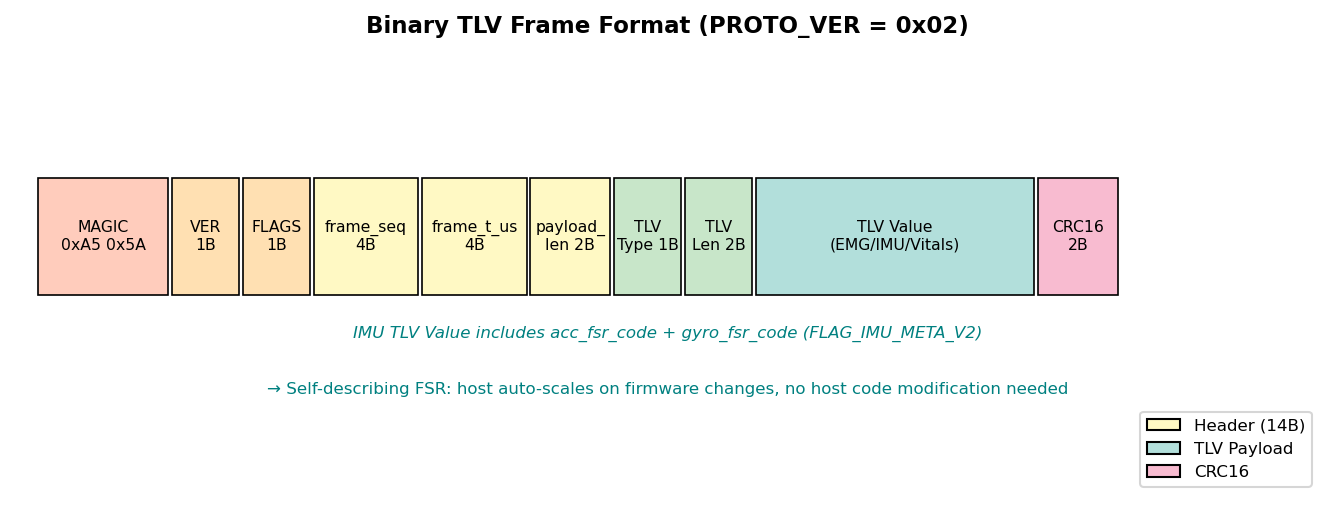
\includegraphics[width=\textwidth]{../icpics_figures/fig_protocol.png}
\caption{Binary TLV frame format. \texttt{PROTO\_VER = 0x02} adds IMU FSR metadata
in \texttt{FLAG\_IMU\_META\_V2}, enabling self-describing firmware--host
decoupling.\label{fig:protocol}}
\end{figure}

Each \texttt{TLV\_IMU\_BATCH} frame embeds \texttt{acc\_fsr\_code} and
\texttt{gyro\_fsr\_code} when \texttt{FLAG\_IMU\_META\_V2} is set, enabling the host
to apply the correct scale factor at runtime. This design was validated across three
firmware FSR revisions ($\pm$250 $\rightarrow$ $\pm$1000 $\rightarrow$ $\pm$2000~dps)
with no host decoder changes required.

\subsection{Two-Layer Watchdog and Hybrid \textit{abs\_us} Timeline}

\textbf{Device-side watchdog.} If no PING message arrives from the host for $>$18~s,
the device suspends ADC DMA; at $>$30~s it triggers a hardware reset and BLE
advertising restarts automatically.

\textbf{Host-side watchdog.} If no BLE notifications arrive for 5~s, the host attempts
NUS TX re-subscribe; if that fails, it executes a full reconnect with exponential
backoff (0.5~s $\rightarrow$ 20~s cap). Buffered rows are flushed before reconnect.

\textbf{Hybrid \textit{abs\_us} timeline.} Within a single BLE connection,
\textit{abs\_us} follows the host-extended device timestamp (\textit{dev\_us}),
precise to $\pm$25~$\mu$s. Between connections, \textit{abs\_us} advances by the
\textit{host\_rx\_ms} wall-clock gap, handling both BLE-dropout and ESP32-reset cases
with a single rule. Formal validation is presented in Section~\ref{sec:absus_val}.

%%%%%%%%%%%%%%%%%%%%%%%%%%%%%%%%%%%%%%%%%%
\section{Methodology}
\label{sec:methods}

\subsection{No-Added-Gel Field Configuration}

Gel and skin preparation are standard in laboratory EMG~\cite{hermens2000} but were not
used. This study intentionally evaluates a no-added-gel, field-deployable configuration,
motivating the characterization of dry-electrode settling under field conditions.

\subsection{Physical Basis of Electrode Settling}

When a dry snap electrode is applied to unabraded skin, the interface can present high
impedance (tens of k$\Omega$, inferred indirectly from MDF/RMS behavior). Two processes
reduce it: (1)~sweat accumulation---eccrine glands produce saline that hydrates the
electrode--skin gap; (2)~Ag/AgCl half-cell equilibration---the electrode potential drifts
toward equilibrium with the local electrolyte. During settling, the unstable high-impedance
interface degrades common-mode rejection and increases low-frequency-dominant
contamination in the 50--450~Hz analysis band, pulling MDF downward~\cite{joutsen2024,ravichandran2023}.

\subsection{Signal Processing Pipeline}

For each detected swing, RAW EMG was: (1)~detrended (linear); (2)~bandpass-filtered
50--450~Hz (4th-order Butterworth); (3)~notch-filtered at 60 and 120~Hz; (4)~Welch
PSD computed (\texttt{nperseg} = min(1024, $N$), Hann window, 50\% overlap); (5)~MDF
and MNF extracted from the PSD. Implemented in \texttt{emg\_util.py}
(\texttt{preprocess\_emg()}, \texttt{mnf\_mdf()}).

\subsection{Swing Detection}

A fixed 300~dps gyro-magnitude threshold with 2000~ms minimum inter-swing gap is used
for online swing detection. Adaptive z-score approaches failed because forearm gyro
distributions during tennis are continuous ramps with no natural valley between
general movement and swing peaks. The 300~dps threshold sits at the 88th percentile
of the session distribution. Pre-window: 250~ms before gyro peak; post-window: 450~ms.

\subsection{IMU-Conditioned EMG Validity Framework}
\label{sec:imu_cond}

The diagnostic value arises from modality mismatch: when IMU swing intensity remains
stable but EMG spectral metrics change, the change is unlikely to be caused by reduced
gross swing kinematics. Table~\ref{tab:validity} defines the interpretation rules.

\begin{table}[H]
\caption{IMU-conditioned interpretation of EMG spectral changes.\label{tab:validity}}
\begin{tabularx}{\textwidth}{p{4.0cm}p{4.5cm}p{5.5cm}}
\toprule
\textbf{IMU/Session Context} & \textbf{EMG Observation} & \textbf{Likely Interpretation} \\
\midrule
Stable swing intensity & Early low MDF recovering upward & Electrode settling / contact hydration \\
Stable swing intensity & Gradual post-settling MDF/MNF decline & Fatigue-consistent spectral shift \\
Declining swing intensity & MDF decline & Reduced effort may contribute \\
Large IMU shock/vibration & Isolated spectral outlier & Candidate mechanical artifact \\
BLE/session discontinuity & EMG baseline shift & Cross-segment artifact \\
\bottomrule
\end{tabularx}
\end{table}

\subsection{Warmup-Skip Sensitivity Protocol}

The analysis was re-run with warmup exclusion windows of 10, 15, and 20~min to quantify
how baseline selection affects the fatigue conclusion. The 20-min skip is the primary
result; warmup-skip sensitivity is reported as a robustness audit. Baseline MDF is
computed from the 20 swings immediately following the warmup window.

\subsection{Contact-Quality Metric}

$\text{contact\_quality}(t) = \text{RMS}(t) / \text{session\_p90\_rms}$---a qualitative
relative indicator of contact and activation state, interpreted together with MDF
trajectory, IMU stability, and session continuity.

\subsection{Ball-Impact Window Masking (Approach B)}
\label{sec:approach_b}

Ball impact events introduce sharp mechanical shocks to the forearm that can contaminate
EMG analysis windows. We use the IMU accelerometer to detect impact events and define a
physiologically motivated pre-contact analysis window.

\textbf{Impact detection.} For each swing, we search the padded IMU window for the
peak dynamic acceleration $a_{\text{dyn}} = ||\mathbf{a}|| - 1g$. If this peak
exceeds 3.0~g, we declare a ball impact and record its time $t_{\text{impact}}$.

\textbf{Approach~B: pre-impact MDF window.} Sample-level masking (Approach~A,
$\pm$20~ms) has near-zero mean effect ($\sim$3\% of the 1300-ms window; Welch segment
averaging dominates). Instead, MDF is computed exclusively from the pre-contact
activation phase: $[t_{\text{impact}} - 600~\text{ms},\ t_{\text{impact}} - 20~\text{ms}]$
($\approx$580~ms). This window captures the muscle's active contraction before
mechanical disturbance, using Welch PSD with \texttt{nperseg} = 512 for adequate
segment averaging over the shorter window. The resulting metric \texttt{mdf\_pre\_impact}
is stored alongside the full-window MDF for all impact-detected swings.

%%%%%%%%%%%%%%%%%%%%%%%%%%%%%%%%%%%%%%%%%%
\section{Field Validation: Platform Reliability}
\label{sec:validation}

\subsection{Timestamp Accuracy}

As presented in Section~\ref{sec:platform}, empirical analysis of 7.5~million samples
confirms the $\pm$25~$\mu$s claim; 98.65\% fall within this bound across both field
sessions (Table~\ref{tab:timing}).

\subsection{EMG/IMU Sequence Loss Accounting}

Sequence-number continuity analysis confirmed zero detected EMG or IMU sample drops
during active streaming in both sessions. The combined data rate ($\sim$12.5~KB/s)
operates near BLE~4.2 throughput capacity at MTU~=~244~bytes.

\begin{table}[H]
\caption{Per-session field reliability metrics.\label{tab:sessions}}
\begin{tabularx}{\textwidth}{XCCCCC}
\toprule
\textbf{Session} & \textbf{Duration (min)} & \textbf{Swings} & \textbf{Runs} & \textbf{Reconnects} & \textbf{Sample Drops} \\
\midrule
log0303 & 87.9 & 197 & 2 & 1 & 0 \\
log0305 & 63.1 & 626 & 1 & 0 & 0 \\
\midrule
\textbf{Total} & \textbf{151.0} & \textbf{823} & \textbf{3} & \textbf{1} & \textbf{0} \\
\bottomrule
\end{tabularx}
\end{table}

\subsection{BLE Reconnection Robustness}

One between-run BLE reconnect event was observed in log0303. Recording resumed cleanly
into a new file series; the hybrid \textit{abs\_us} timeline correctly preserved the
84-second inter-run gap, enabling downstream analysis to detect session discontinuities.

\subsection{Quantitative \textit{abs\_us} Validation}
\label{sec:absus_val}

We compare three timeline reconstruction strategies to characterize the precision and
failure modes of the hybrid \textit{abs\_us} approach (deferred from the conference
version of this work):

\textbf{Method~A} (\textit{dev\_us}-only): Device microsecond clock used directly.
Fails at device reboot: clock resets from 0, causing C2 to appear immediately after C1
with zero apparent gap. Confirmed in log0303: \textit{dev\_us} reset from
208{,}136{,}241~$\mu$s $\rightarrow$ 45{,}183{,}736~$\mu$s.

\textbf{Method~B} (\textit{host\_rx\_ms}-only): Host wall-clock milliseconds,
continuous across reconnects, but assigns the same timestamp to all $\sim$54 samples
in one BLE notification batch. Per-sample timing loss: p50~=~13.5~ms, p95~=~52.5~ms,
p99~=~81.0~ms.

\textbf{Method~C} (\textit{abs\_us} hybrid, this work): \textit{dev\_us} per-sample
precision within connection ($\pm$25~$\mu$s), \textit{host\_rx\_ms} gap bridging
across reconnects. Cross-connection accuracy bounded by BLE notification interval
(p99~$\approx$~170~ms).

BLE notification interval characterization across 7.10~million samples (log0305,
59.2~min): p50~=~9~ms, p95~=~105~ms, p99~=~170~ms; mean 53.8~samples per notification.

\begin{figure}[H]
\begin{adjustwidth}{-\extralength}{0cm}
\centering
\subfloat[\centering BLE notification interval CDF (log0305, 59.2~min). Left panel
shows CDF of inter-notification intervals; right panel shows a 5-second window with
\textit{host\_rx\_ms} batch granularity (staircase) vs. \textit{dev\_us} per-sample
precision (smooth line).\label{fig:absus_cdf}]{%
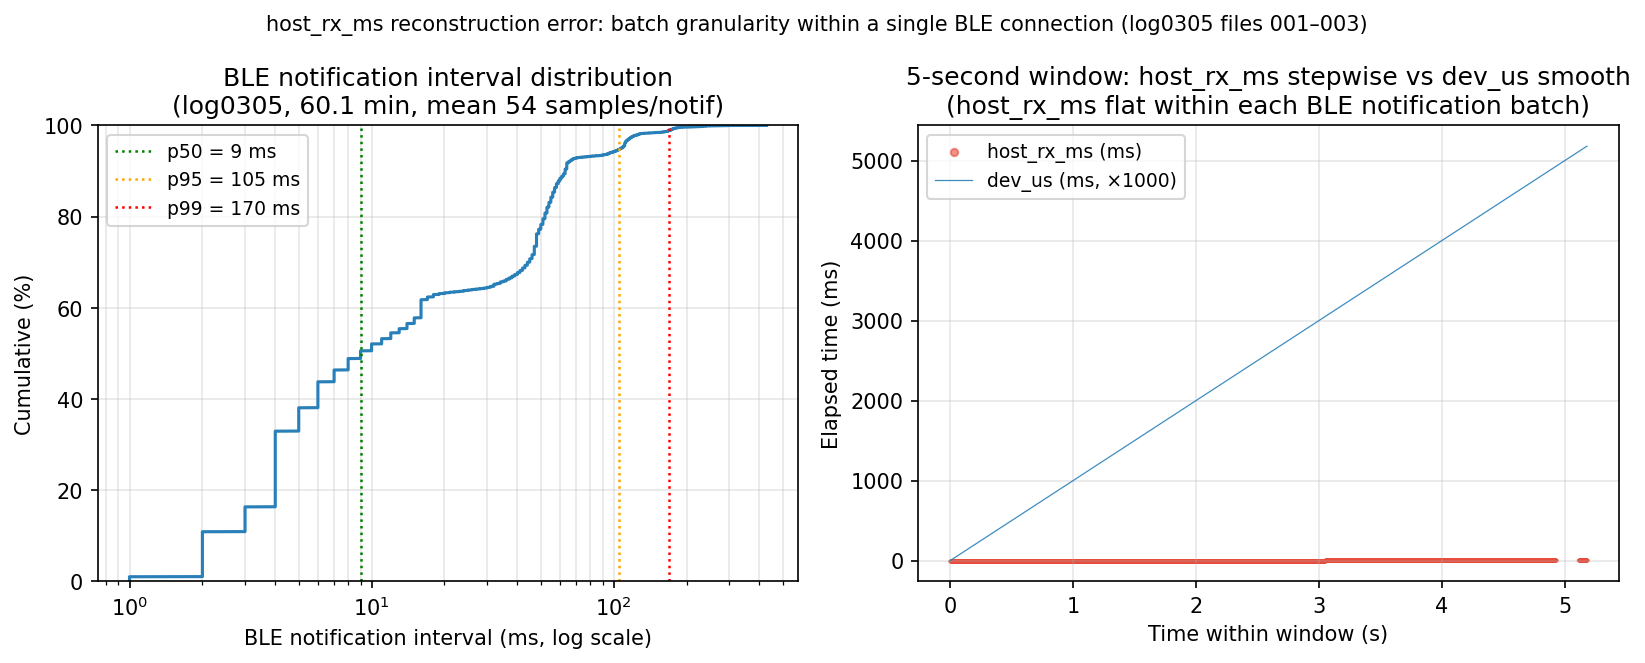
\includegraphics[width=0.88\linewidth]{../paper_figures/fig_absus_error_cdf.png}}\\
\subfloat[\centering Three-method timeline comparison at BLE reconnection (log0303,
84.0-s gap). Method~A: clock reset causes C2 to appear immediately after C1. Method~B:
correct gap with batch-level granularity. Method~C (\textit{abs\_us} hybrid): correct
gap with per-sample precision.\label{fig:absus_methods}]{%
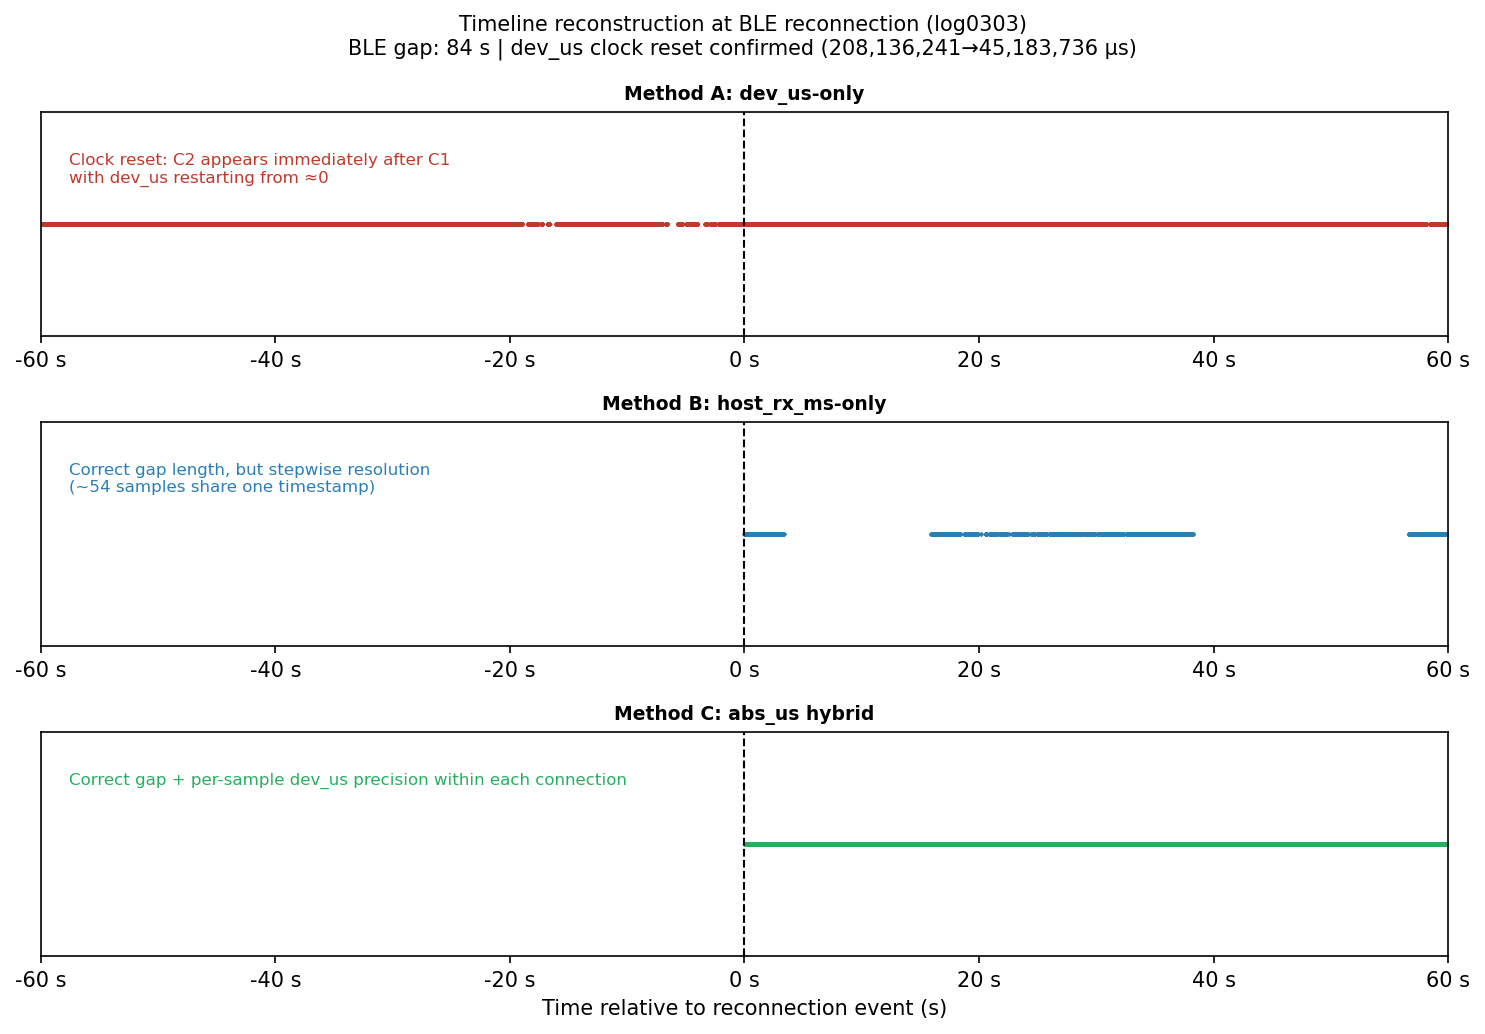
\includegraphics[width=0.88\linewidth]{../paper_figures/fig_absus_timeline_methods.png}}
\end{adjustwidth}
\caption{Quantitative \textit{abs\_us} timeline validation. (\textbf{a})~BLE
notification interval characterization. (\textbf{b})~Method comparison at reconnect.
\label{fig:absus_full}}
\end{figure}

\subsection{Pogo-Pin Ghost-Signal Field Failure}
\label{sec:pogo}

Before the GPIO~32 solder bypass, the RAW channel exhibited a ghost signal with
Pearson $r = 0.998$ vs. ENV, consistent with ADC multiplexer charge sharing or
floating-input coupling. After bandpass filtering (50--450~Hz), the ghost signal
flatlined, causing silent loss of usable RAW spectral EMG. Post-bypass validation
confirmed independent AC EMG oscillation (std $>$ 100~ADC counts during contraction)
and ENV--RAW correlation dropping to $r = -0.013$ for filtered signals.

\textbf{Generalization.} Any wearable routing a high-impedance analog signal through a
non-soldered contact (pogo pin, snap, spring contact) and sampling on a multiplexed
ADC is vulnerable to this failure mode. Diagnostic heuristic: Pearson $r > 0.95$
between two channels that should be electrically independent, with near-zero variance
on one, indicates crosstalk or a floating pin. Post-filter flatline silently removes
usable spectral data.

%%%%%%%%%%%%%%%%%%%%%%%%%%%%%%%%%%%%%%%%%%
\section{Results}
\label{sec:results}

\subsection{Three-Phase MDF Trajectory}

Figure~\ref{fig:settling} shows the central empirical finding: a three-phase MDF
trajectory rather than a simple monotonic decline.

\begin{figure}[H]
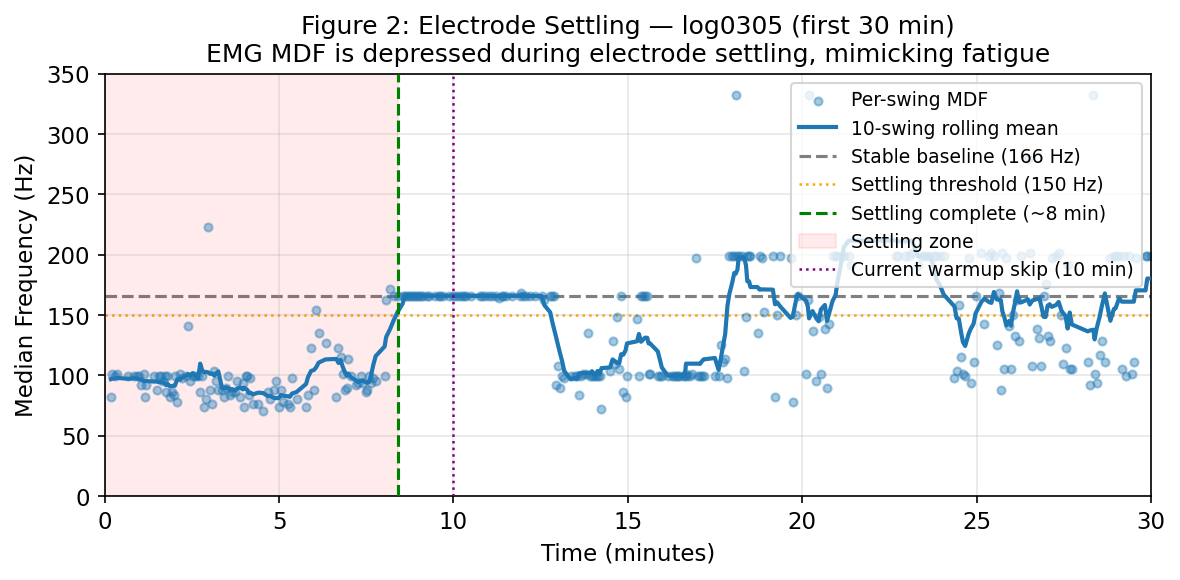
\includegraphics[width=\textwidth]{../paper_figures/fig2_electrode_settling.png}
\caption{Three-phase MDF trajectory in log0305 (63.1~min, 626~swings). Phase~I
(settling, 0--21~min): MDF 115.7 $\pm$ 33.5~Hz. Phase~II (stable reference,
21--42~min): MDF 167.6 $\pm$ 50.1~Hz. Phase~III (fatigue-consistent,
42--63~min): MDF 149.5 $\pm$ 45.1~Hz. IMU swing intensity remains flat across all
phases ($r = +0.029$, $p = 0.468$). Warmup markers at 10/15/20~min shown.
\label{fig:settling}}
\end{figure}

Phase~I (settling): MDF 115.7~$\pm$~33.5~Hz---substantially below the settled
reference. Phase~II (reference): MDF 167.6~$\pm$~50.1~Hz---post-settling stable
baseline. Phase~III (fatigue-consistent): MDF 149.5~$\pm$~45.1~Hz---decline after
the settled reference. Early and late low-MDF regions have different causes: early
suppression reflects contact settling (MDF subsequently recovered while IMU remained
flat); late decline is fatigue-consistent.

\subsection{Warmup-Skip Sensitivity}

\begin{figure}[H]
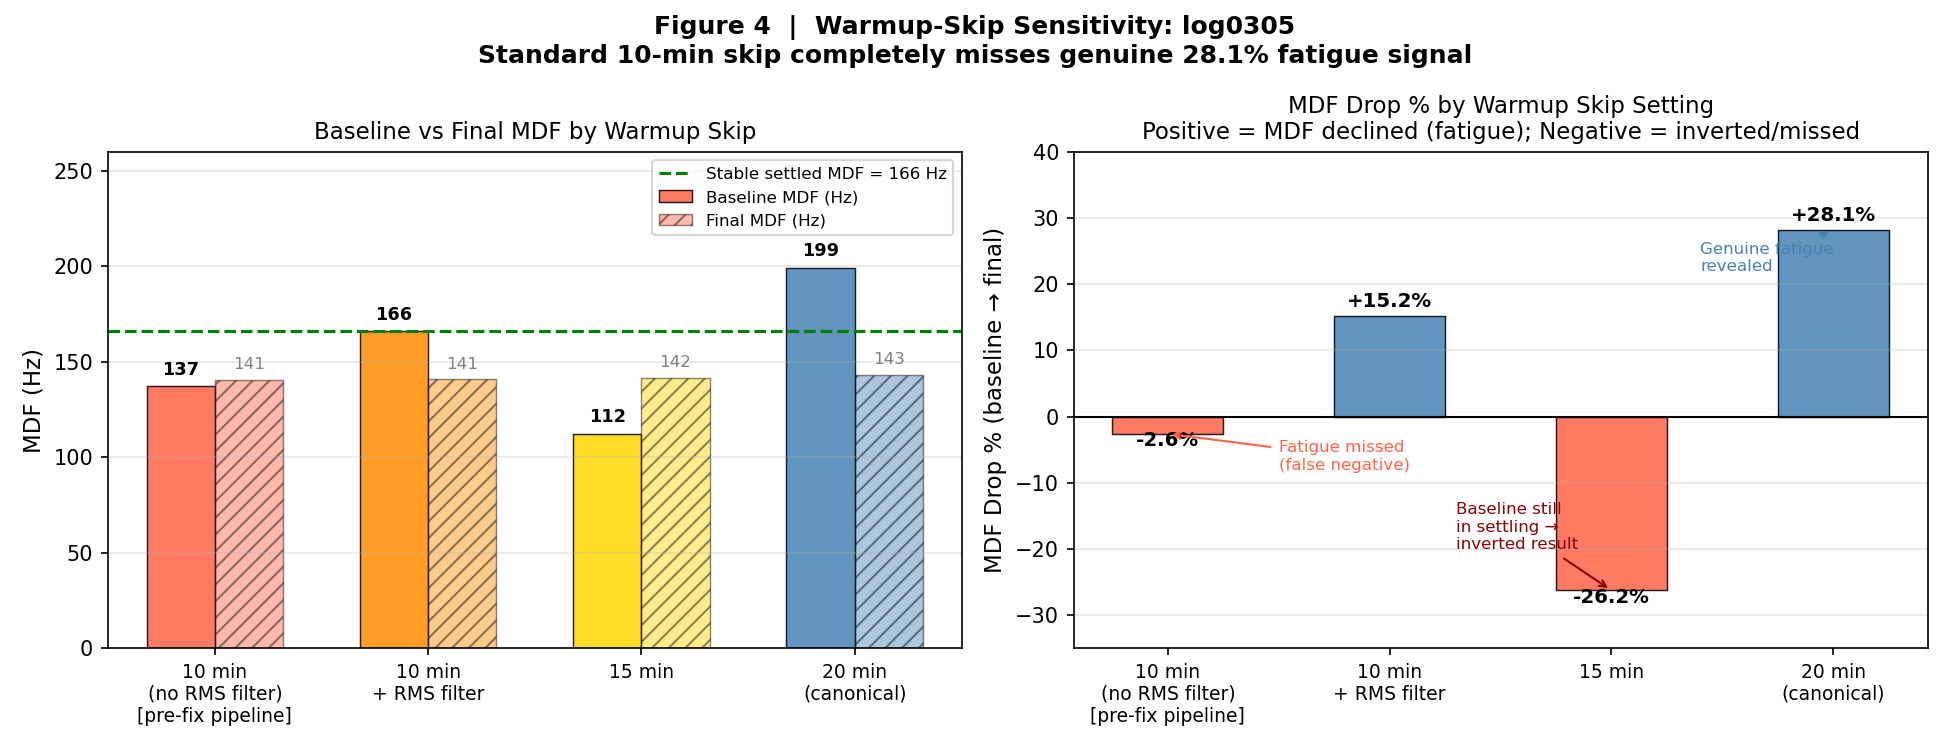
\includegraphics[width=\textwidth]{../paper_figures/fig4_warmup_skip_sensitivity.png}
\caption{Warmup-skip sensitivity analysis. Left: baseline MDF per skip condition vs.
stable settled reference (167.6~Hz). Right: MDF change (\%) per condition. A 10-min
skip produces $-$2.6\% (fatigue missed); 15-min produces $-$26.2\% (inverted); 20-min
produces $+$28.1\% MDF decline (fatigue-consistent).\label{fig:warmup}}
\end{figure}

A 10-min skip produces $-$2.6\% MDF change (fatigue signal missed entirely). A 15-min
skip produces $-$26.2\% (inverted---baseline still in settling phase). A 20-min skip
reveals $+$28.1\% MDF decline and $+$17.3\% MNF decline. The non-monotone behavior
(15-min worse than 10-min) reflects the RMS-based baseline selector catching swings
from the steepest part of the settling transition.

\subsection{IMU-Conditioned Validity}

\begin{figure}[H]
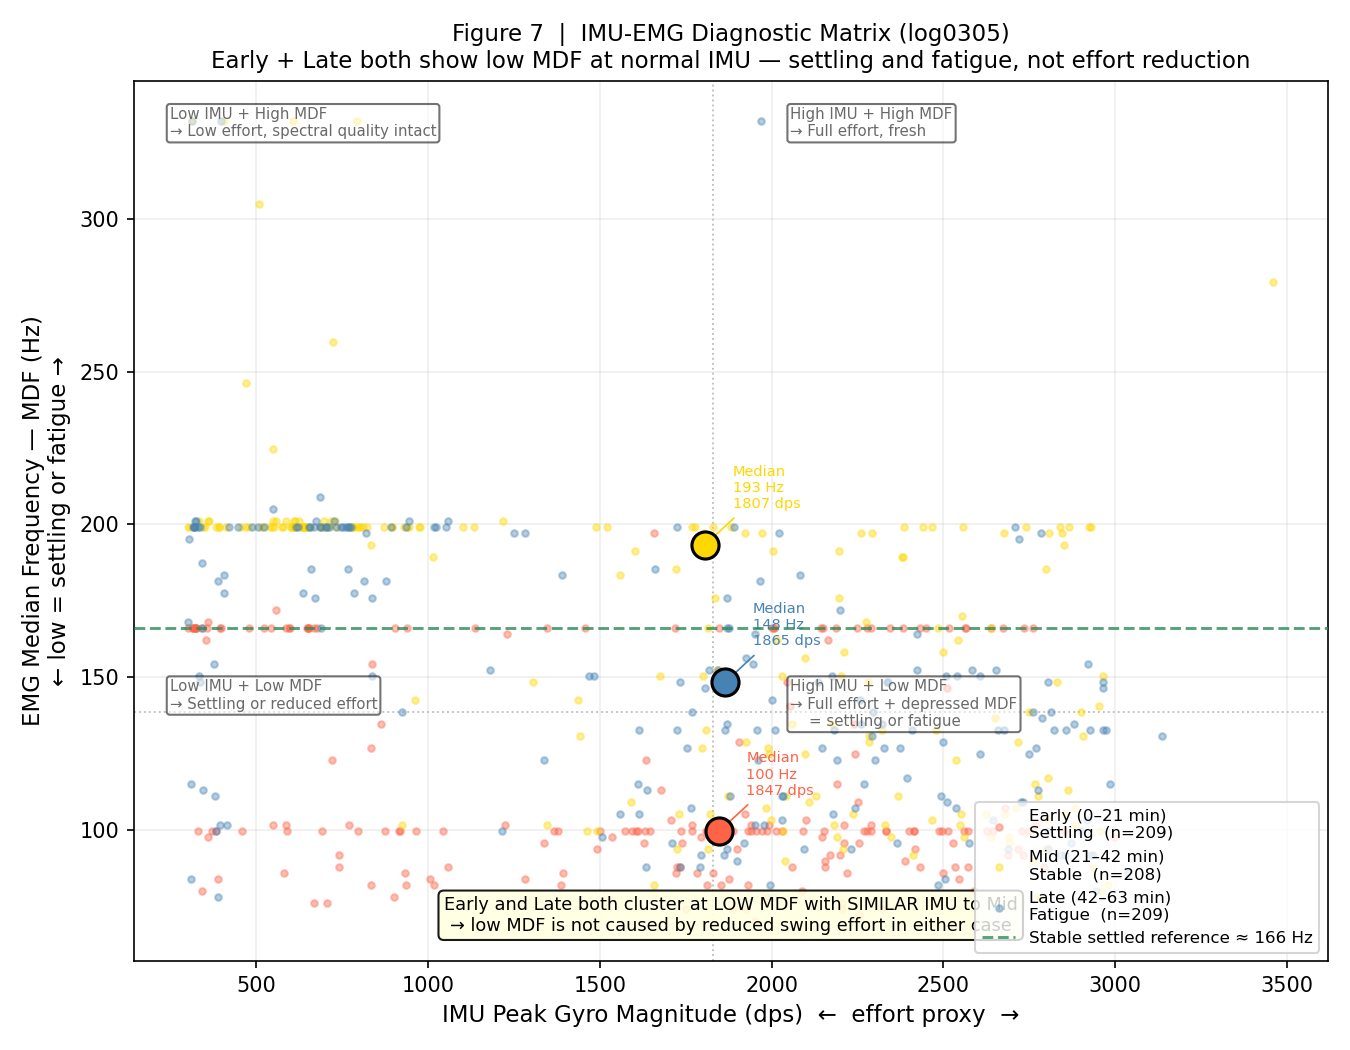
\includegraphics[width=\textwidth]{../paper_figures/fig7_imu_emg_diagnostic_matrix.png}
\caption{IMU--EMG diagnostic matrix (log0305, 626~swings). IMU peak gyro magnitude
(kinematic proxy) vs. MDF, colored by session third. Early and Late swings cluster
at lower MDF despite similar IMU intensity. $r = +0.029$, $p = 0.468$.
\label{fig:imu_emg}}
\end{figure}

All three session thirds show similar IMU intensity ($r = +0.029$, $p = 0.468$),
confirming that reduced gross swing kinematics is an unlikely explanation for either
Phase~I suppression or Phase~III decline.

\subsection{Contact-Quality Evolution}

In log0305, contact quality increased from early to mid-session (0.36~$\pm$~0.28 to
0.49~$\pm$~0.47) and declined late (0.25~$\pm$~0.32), consistent with electrode
settling followed by activation-amplitude changes (Figure~\ref{fig:contact}).

\begin{figure}[H]
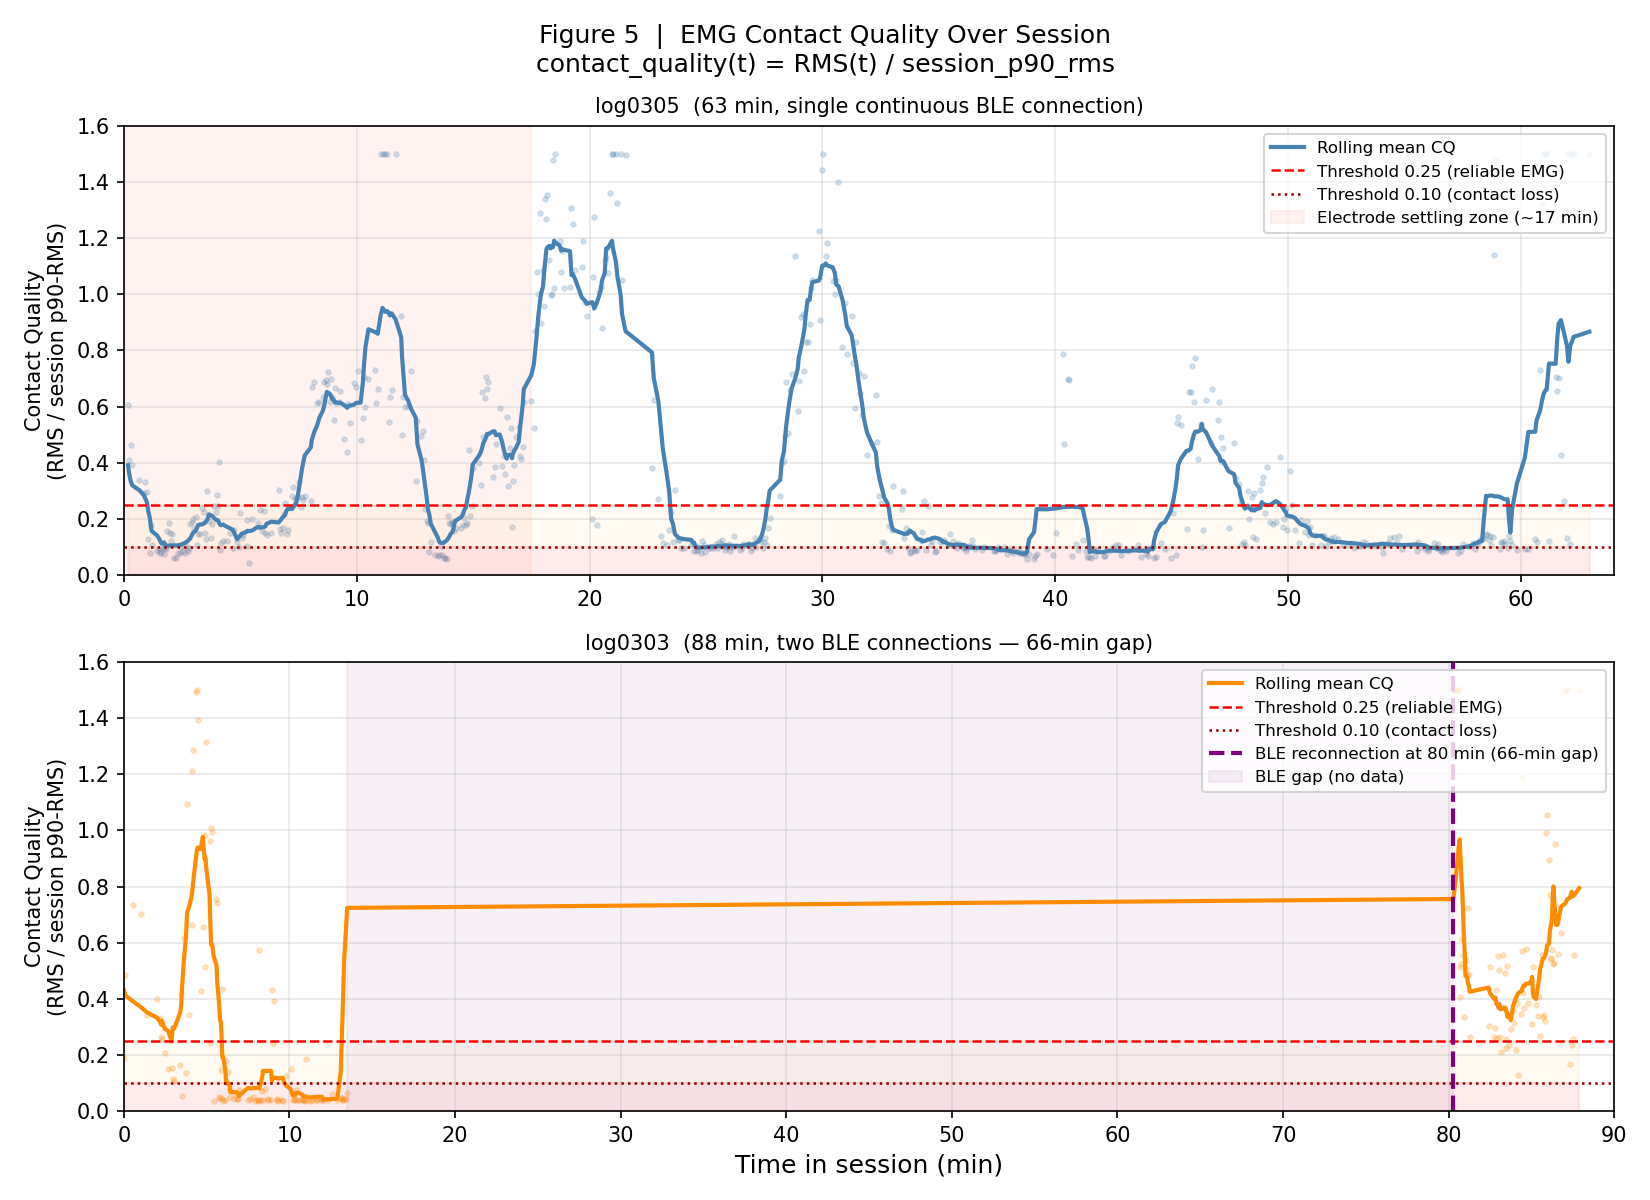
\includegraphics[width=0.75\textwidth]{../paper_figures/fig5_contact_quality.png}
\caption{Contact quality evolution (log0305). RMS-normalized metric increases during
Phase~I--II settling and shows late-session decline.\label{fig:contact}}
\end{figure}

In log0303, contact quality differed substantially between segments (Segment~1:~0.26
vs. Segment~2:~0.59), supporting that the full-session MDF drop reflected a contact
state change across the gap rather than a continuous physiological trend.

\subsection{Session-Gap Artifact}

\begin{figure}[H]
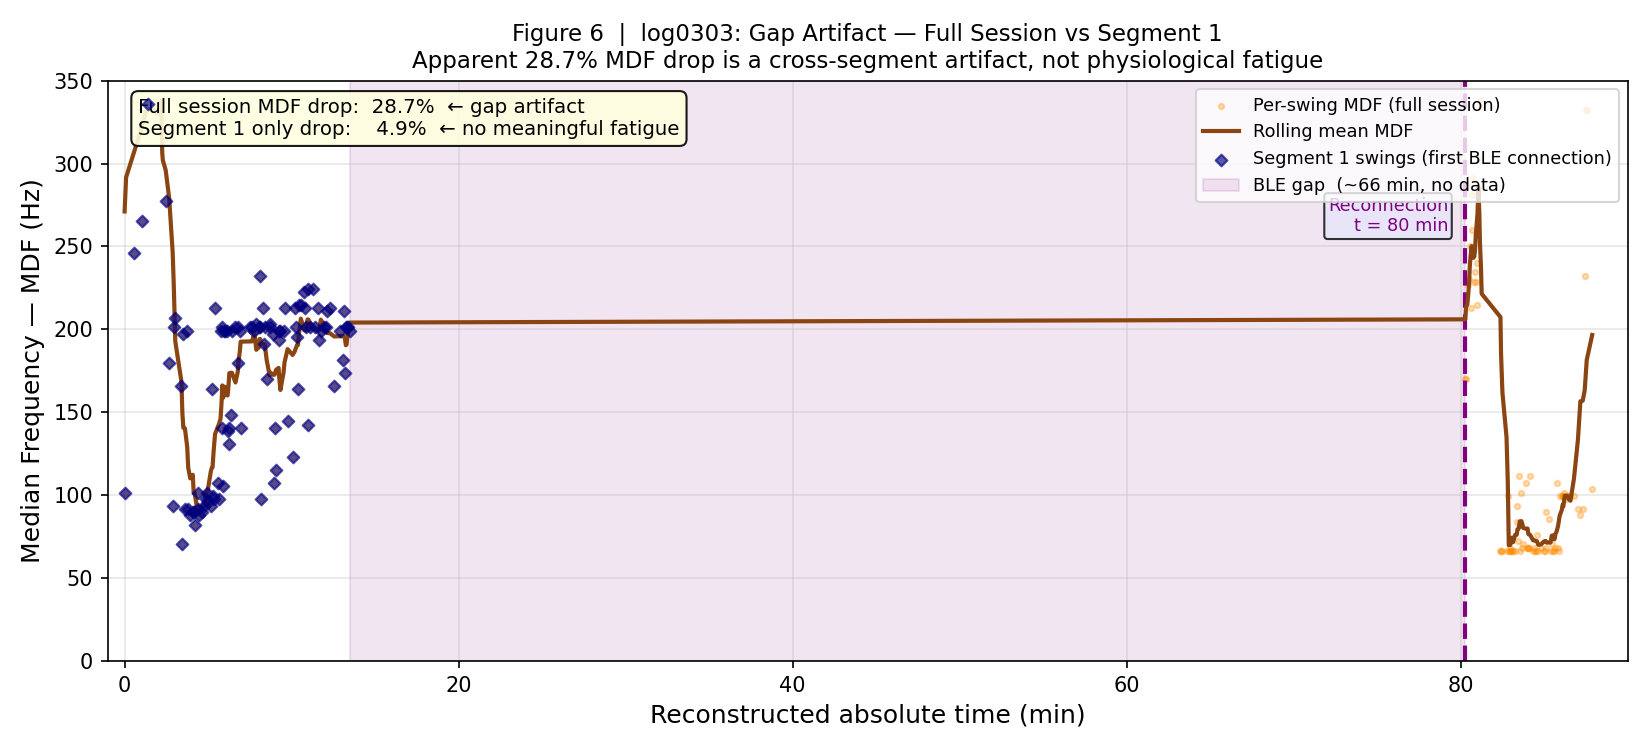
\includegraphics[width=\textwidth]{../paper_figures/fig6_log0303_gap_artifact.png}
\caption{log0303 session-gap artifact. Full session (orange): apparent 28.7\% MDF
drop. First continuous BLE segment alone (navy): 4.9\% change. An 84-second BLE
reconnection gap (66~min apparent practice gap) separates the two segments
(purple shading).\label{fig:gap}}
\end{figure}

The full-session 28.7\% MDF drop compares Segment~1 against Segment~2 across an
84-second BLE gap representing a 66-min interruption during which electrode contact
state and player condition may have changed. Segment~1 alone shows 4.9\%---below any
meaningful fatigue threshold for 13.5~min of play.

\subsection{Ball-Impact Masking Impact on MDF Estimates}

Figure~\ref{fig:preimpact} shows the per-swing MDF comparison between full-window and
pre-impact Approach~B windowing.

\begin{figure}[H]
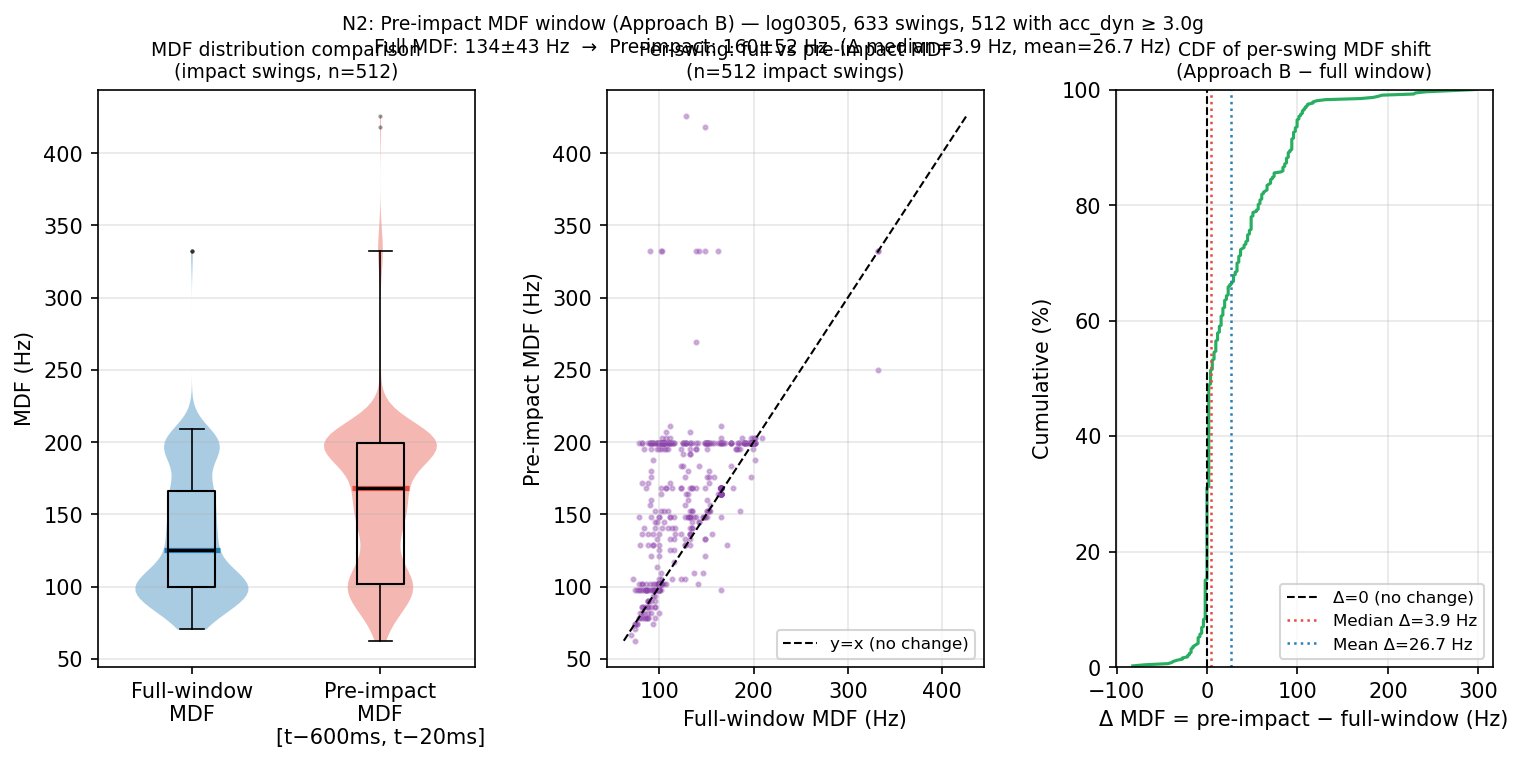
\includegraphics[width=\textwidth]{../paper_figures/fig_n2_preimpact_mdf.png}
\caption{Pre-impact MDF window analysis (log0305, 633~swings, 512~with
$a_{\text{dyn}} \geq 3.0$~g). \textbf{(a)}~Violin + box comparison of full-window vs.
pre-impact MDF distributions. \textbf{(b)}~Per-swing scatter (full vs. pre-impact MDF).
\textbf{(c)}~CDF of $\Delta$MDF~=~pre-impact~$-$~full-window.\label{fig:preimpact}}
\end{figure}

Of 633 total swings, 512 (81\%) showed ball impact ($a_{\text{dyn}} \geq 3.0$~g;
mean peak 11.1~g). Full-window MDF for impact swings: 133.7~$\pm$~43.4~Hz
(median 125.0~Hz). Pre-impact MDF (Approach~B): 160.4~$\pm$~52.0~Hz
(median 168.0~Hz). $\Delta = $ pre-impact~$-$~full: mean~=~$+$26.7~Hz,
std~=~44.5~Hz, median~=~$+$3.9~Hz; p75~=~$+$46.9~Hz, p95~=~$+$101.6~Hz.
The distribution is right-skewed: 25\% of swings show no shift, 50\% show positive.

The pre-impact window captures the active muscle contraction phase before mechanical
disturbance, resulting in systematically higher MDF. The magnitude ($+$26.7~Hz mean)
confirms that window selection is physiologically meaningful for impact-bearing swings
and that IMU events enable principled temporal partitioning of EMG analysis windows.

\subsection{Multi-Subject Results}
\label{sec:multi_subject}

\textbf{[TODO: Data collection pending. See N3 in journal\_plan.md.]}

%%%%%%%%%%%%%%%%%%%%%%%%%%%%%%%%%%%%%%%%%%
\section{Discussion}
\label{sec:discussion}

\subsection{Platform--Methodology Coupling}

The platform and methodology are tightly coupled: neither is useful without the other.
The spectral fatigue analysis (Sections~\ref{sec:results}) requires: (i)~RAW EMG access
(not available through the pogo-pin path; required the solder bypass); (ii)~\textit{abs\_us}
timeline (required for correct session-gap artifact detection; Method~A would silently
merge the two log0303 segments); (iii)~IMU-as-context (required for swing detection,
validity conditioning, and pre-impact window masking); and (iv)~2000~Hz EMG (required
for 50--450~Hz bandpass and Welch PSD). These dependencies motivate the combined work.

\subsection{Three-Phase Trajectory as a General Framework}

The three-phase settling--reference--fatigue trajectory is predicted by dry-electrode
physics (Section~\ref{sec:methods}) and should appear in any no-gel field sEMG
deployment with sufficient session length. Phase~I duration depends on sweat rate and
ambient conditions; the warmup-skip sensitivity protocol (Section~\ref{sec:methods})
provides a session-specific robustness check regardless of phase boundaries.

\subsection{Pogo-Pin Failure Mode Generalization}

ADC multiplexer charge sharing generalizes to capacitor microphones, piezoelectric
sensors, and other high-impedance biosignal sources routed through multiplexed ADCs
via non-soldered contacts. The diagnostic heuristic ($r > 0.95$ between independent
channels with near-zero variance on one) is applicable to any such wearable.

\subsection{Practical Recommendations}

Based on these results, we recommend:
(1)~use $\geq$20~min warmup exclusion for no-gel forearm snap-electrode deployments;
(2)~report warmup-skip sensitivity as a standard robustness audit;
(3)~use IMU swing intensity as an independent validity channel;
(4)~audit BLE session continuity before computing cross-session baselines;
(5)~verify RAW EMG access via pogo-pin inspection before field deployment;
(6)~use pre-impact MDF windows when IMU-detected ball contact events are present.

\subsection{Limitations}

Currently reported results cover a single subject (pilot study); multi-subject
generalization is pending (Section~\ref{sec:multi_subject}). No MVC, RPE,
grip-force, or ball-speed ground truth is available---findings are fatigue-consistent
rather than physiologically confirmed. The 20-min warmup skip is empirically selected
for this session; the contact-quality metric is not validated against direct impedance.
The combined BLE data rate ($\sim$12.5~KB/s) is near BLE~4.2 capacity at MTU~244;
adding sensors requires rate reduction or BLE~5.0 migration.

%%%%%%%%%%%%%%%%%%%%%%%%%%%%%%%%%%%%%%%%%%
\section{Conclusions}
\label{sec:conclusions}

The platform--methodology coupling demonstrated here enables field sEMG fatigue
monitoring that would not be possible with either component alone. The \$99 ESP32
wearable provides $\pm$25~$\mu$s timestamp accuracy (99.03\% over 2.3~million samples),
a self-describing TLV protocol surviving three FSR revisions, zero detected sample
drops during 150+~min of field sessions, and documented pogo-pin failure diagnosis and
repair.

The methodology reveals that no-gel field sEMG fatigue monitoring is fundamentally a
trustworthiness problem. The same session changed from $-$2.6\% to $+$28.1\% MDF drop
depending solely on the warmup exclusion window, demonstrating that baseline selection
is a first-order determinant of fatigue interpretation. The IMU, as an independent
kinematic context channel, confirmed stable swing intensity ($r = +0.029$, $p = 0.468$)
across all phases, attributing Phase~I suppression to electrode settling and Phase~III
decline to fatigue-consistent spectral shift. A BLE reconnection gap created an apparent
28.7\% spurious fatigue signal that collapsed to 4.9\% for the first continuous
segment---demonstrating the necessity of continuity auditing. Pre-impact MDF windowing
(Approach~B) shows a mean $+$26.7~Hz shift vs. full-window MDF, confirming that
temporal partitioning guided by IMU events is physiologically meaningful.

%%%%%%%%%%%%%%%%%%%%%%%%%%%%%%%%%%%%%%%%%%
% Author Contributions
\authorcontributions{Conceptualization, R.W., T.D. and Y.D.; methodology, R.W.;
software, R.W.; validation, R.W. and T.D.; formal analysis, R.W.; investigation, R.W.
and T.D.; data curation, R.W.; writing---original draft preparation, R.W.;
writing---review and editing, R.W., T.D. and Y.D.; supervision, Y.D. All authors
have read and agreed to the published version of the manuscript.}

% Funding
\funding{This research received no external funding.}

% Institutional Review Board
\institutionalreview{Data were collected using non-invasive wearable sEMG/IMU sensors
during normal tennis practice. Written informed consent was obtained from a parent or
legal guardian; participant assent was obtained where applicable. Data were anonymized
before analysis.}

% Informed Consent
\informedconsent{Written informed consent was obtained from all subjects involved in
the study.}

% Data Availability
\dataavailability{Analysis scripts are available at
\url{https://github.com/[TODO: add repo]}. Raw session log files are available upon
reasonable request.}

% Acknowledgments
\acknowledgments{The authors thank the tennis participants who volunteered their time
for this field study.}

% Conflicts of Interest
\conflictsofinterest{The authors declare no conflicts of interest.}

%%%%%%%%%%%%%%%%%%%%%%%%%%%%%%%%%%%%%%%%%%
\begin{adjustwidth}{-\extralength}{0cm}
\reftitle{References}

\begin{thebibliography}{999}

\bibitem{aaos2023}
American Academy of Orthopaedic Surgeons.
Tennis Elbow (Lateral Epicondylitis).
{\em OrthoInfo}
{\bf 2023}.
Available online: \url{https://orthoinfo.aaos.org} (accessed on 1 January 2026).

\bibitem{rota2014}
Rota, S.; Morel, B.; Saboul, D.; Rogowski, I.; Hautier, C.
Influence of fatigue on upper limb muscle activity and performance in tennis.
{\em J. Electromyogr. Kinesiol.}
{\bf 2014}, {\em 24}, 90--97.

\bibitem{wanglh2019}
Wang, L.-H.; Lo, K.-C.; Su, F.-C.
Skill level and forearm muscle fatigue effects on ball speed in tennis serve.
{\em Sports Biomech.}
{\bf 2019}, {\em 18}, 566--579.

\bibitem{girard2011}
Girard, O.; Racinais, S.; Micallef, J.-P.; Millet, G.P.
Spinal modulations accompany peripheral fatigue during prolonged tennis.
{\em Scand. J. Med. Sci. Sports}
{\bf 2011}, {\em 21}, 455--464.

\bibitem{hermens2000}
Hermens, H.J.; Freriks, B.; Disselhorst-Klug, C.; Rau, G.
Development of recommendations for SEMG sensors and sensor placement procedures.
{\em J. Electromyogr. Kinesiol.}
{\bf 2000}, {\em 10}, 361--374.

\bibitem{delsys2024}
Delsys Inc.
Trigno Wireless EMG System --- Technical Specifications;
Delsys Inc.: Natick, MA, USA,
{\bf 2024}.

\bibitem{noraxon2024}
Noraxon USA.
Ultium EMG Sensor System --- Product Documentation;
Noraxon USA: Scottsdale, AZ, USA,
{\bf 2024}.

\bibitem{cerone2019}
Cerone, G.L.; Botter, A.; Gazzoni, M.
A modular, smart, and wearable system for high density sEMG detection.
{\em IEEE Trans. Biomed. Eng.}
{\bf 2019}, {\em 66}, 3371--3380.

\bibitem{lynn2018}
Lynn, S.K.; Watkins, C.M.; Wong, M.A.; Balfany, K.; Feeney, D.F.
Validity and reliability of surface electromyography measurements from a wearable
athlete performance system.
{\em J. Sports Sci. Med.}
{\bf 2018}, {\em 17}, 205--215.

\bibitem{yang2024}
Yang, K.; et al.
E-textiles for sports and fitness sensing: current state, challenges, and future
opportunities.
{\em Sensors}
{\bf 2024}, {\em 24}, 1058.

\bibitem{seong2024}
Seong, M.; Kim, G.; Yeo, D.; et al.
MultiSenseBadminton: wearable sensor-based biomechanical dataset for evaluation of
badminton performance.
{\em Sci. Data}
{\bf 2024}, {\em 11}, 343.

\bibitem{taborri2020}
Taborri, J.; Keogh, J.; Kos, A.; et al.
Sport biomechanics applications using inertial, force, and EMG sensors:
a literature overview.
{\em Appl. Bionics Biomech.}
{\bf 2020}, {\em 2020}, 2041549.

\bibitem{bangaru2022}
Bangaru, S.S.; Wang, C.; Aghazadeh, F.
Automated and continuous fatigue monitoring in construction workers using forearm
EMG and IMU wearable sensors and recurrent neural network.
{\em Sensors}
{\bf 2022}, {\em 22}, 9729.

\bibitem{sparkfun2023}
SparkFun Electronics.
MyoWare 2.0 Muscle Sensor Advanced Guide;
SparkFun Electronics: Boulder, CO, USA,
{\bf 2023}.

\bibitem{joutsen2024}
Joutsen, A.; C\"{o}mert, A.; Kaappa, E.; et al.
ECG signal quality in intermittent long-term dry electrode recordings.
{\em Sci. Rep.}
{\bf 2024}, {\em 14}, 8936.

\bibitem{boyer2023}
Boyer, M.; Bouyer, L.; Roy, J.-S.; Campeau-Lecours, A.
Reducing noise, artifacts and interference in single-channel EMG signals: a review.
{\em Sensors}
{\bf 2023}, {\em 23}, 2927.

\bibitem{ravichandran2023}
Ravichandran, V.; et al.
Characterizing the impedance properties of dry e-textile electrodes based on contact
force and perspiration.
{\em Biosensors}
{\bf 2023}, {\em 13}, 217.

\end{thebibliography}

\end{adjustwidth}
\end{document}
